\textbf{Description:} This sequence diagram describes how students view their daily events from the scheduling system. 
First, the system gets data from the database and checks it with Google Calendar. Then, when a lecturer or university updates a new daily event, which is in conflict with its database, the system gets conflict data and saves it to the database. 
Finally, the students see the new event and send notification about the conflicts. \\

\noindent \textbf{Pre-conditions:} 
    \begin{itemize}
        \item Students are logged in.
        \item Students have access to the Schedule Page.
        \item System connects to the database and Google Calendar.
    \end{itemize}

\noindent \textbf{Post-conditions:}
\begin{itemize}
    \item System connects to the database and Google Calendar.
    \item System sends a notification of an update daily event.
    \item The database is updated with the new data from Google Calendar.
\end{itemize}

\subsubsection{StudyBuddy Sequence Diagram}
\textbf{Description:} This sequence diagram describes how students connect with others. 
When students access the Study Buddy page, they see a list of recommended study buddies, which is generated by a model based on their database. 
Students can communicate with the others by using 2 features: message and calling. \\

\noindent \textbf{Pre-conditions:} 
    \begin{itemize}
        \item Students are logged in.
        \item Students have access to the Study Buddy page.
        \item Students are logged in to an SIP account.
        \item Both students are connected to each other.
    \end{itemize}
\noindent \textbf{Post-conditions:}
\begin{itemize}
    \item Students view a list of recommended study buddies.
    \item Students view and edit their profiles.
    \item Students can contact each other while using the message and call of the application.
\end{itemize}

\subsubsection{Real-Time Notification Sequence Diagram}
\begin{figure}[H]
    \centering
    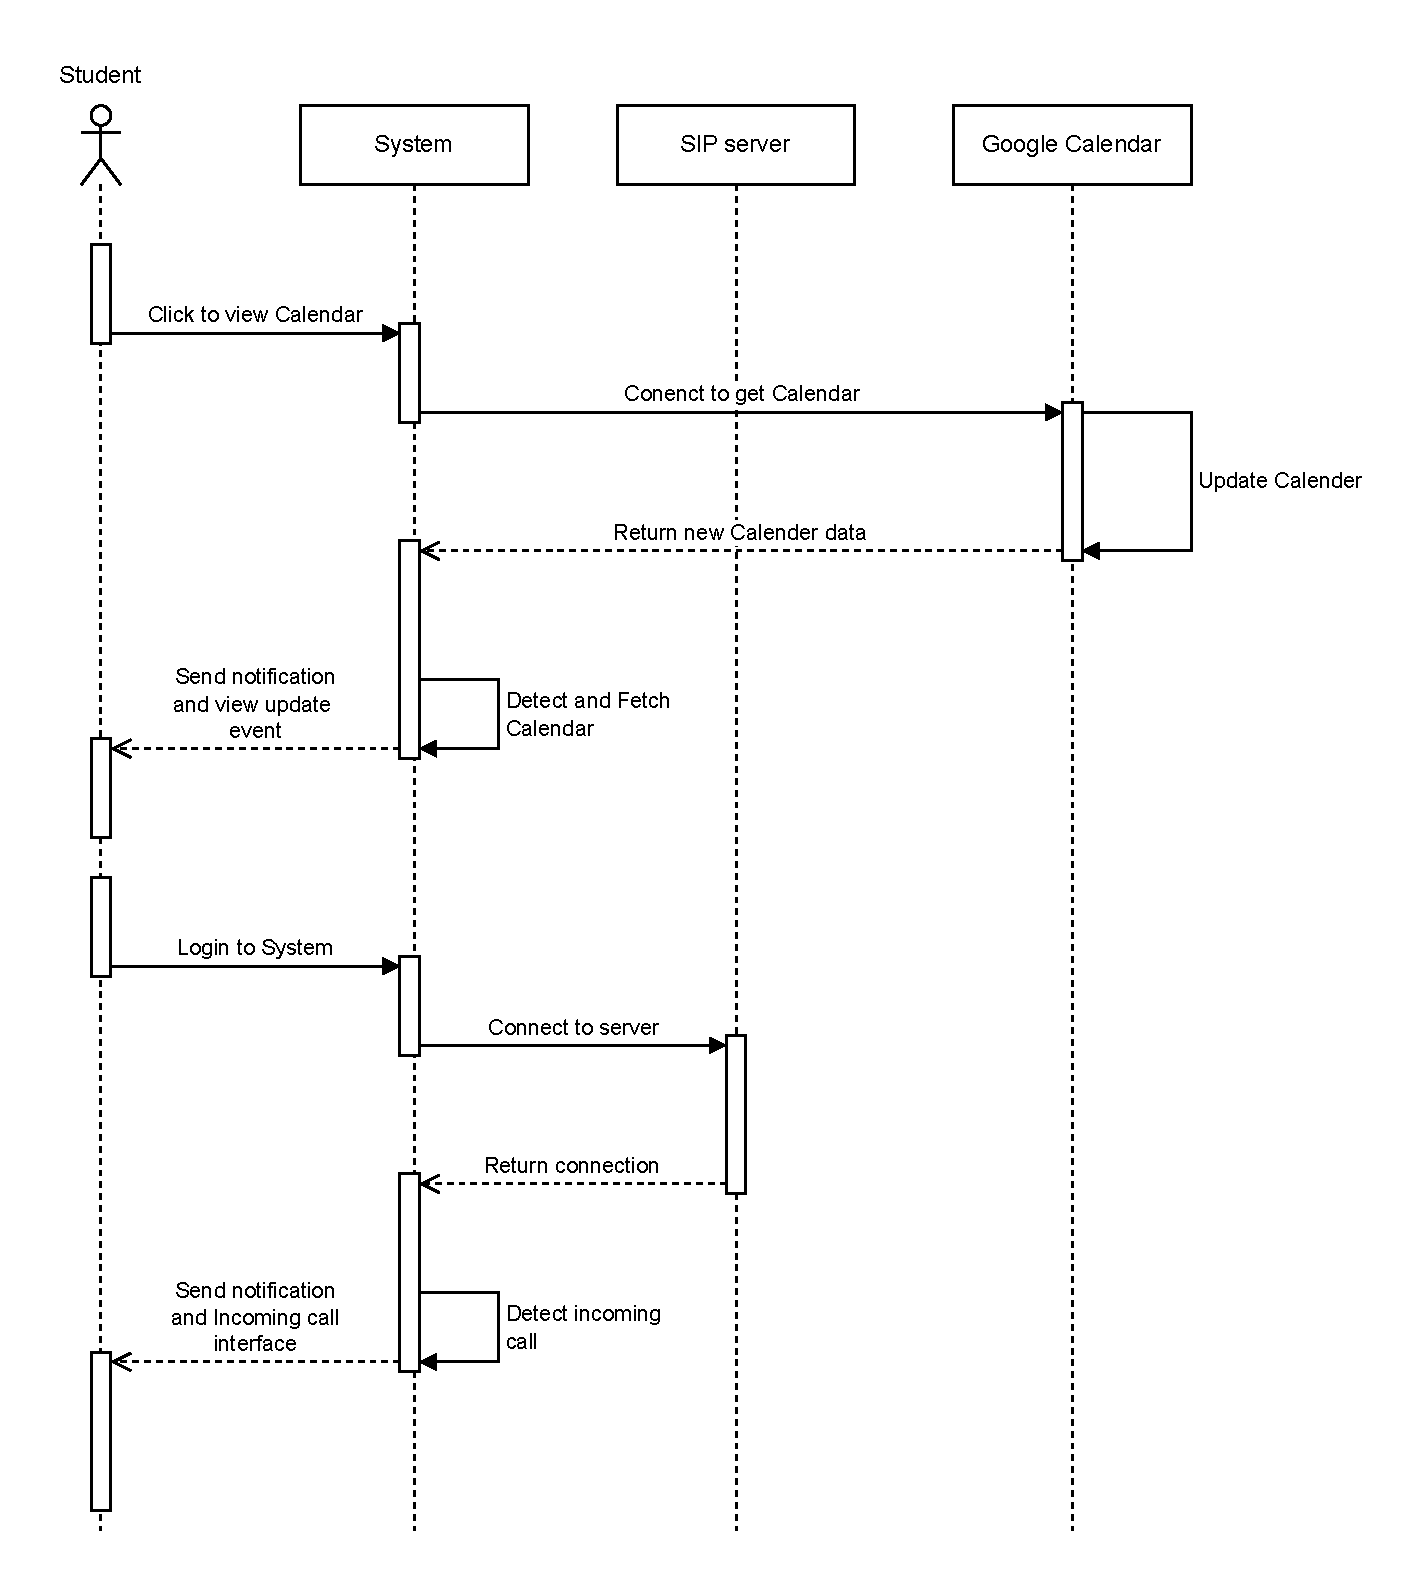
\includegraphics[width=0.7\textwidth]{image/Real-timeNotification.pdf} 
    \caption{Real Time Notification sequence diagram}
    \label{fig:noti_sequence}
\end{figure}

\textbf{Description:} This sequence diagram describes how systems send notifications to students to view update events in the calendar and incoming calls from other students. 
First, the system connects to Google Calendar and SIP Server. 
Then, if the calendar changes, systems detect the calendar, which is updated by the lecturer or university, fetch the calendar and send notification. 
Second, the system connects to the SIP Server. When a student calls another, the system detects that and sends notification to the student. \\

\noindent \textbf{Pre-conditions:} 
    \begin{itemize}
        \item Students are logged in.
        \item System connected to both SIP Server and Google Calendar.
    \end{itemize}
\noindent \textbf{Post-conditions:}
\begin{itemize}
    \item Students receive notification about the update calendar.
    \item Students receive a notification and can access the incoming call interface.
\end{itemize}
